\documentclass{article}
% The file ijcai15.sty is the style file for IJCAI-15 (same as ijcai07.sty).
\usepackage{ijcai15}

% Use the postscript times font!
\usepackage{times}

%my stuff
\usepackage{amssymb}
\usepackage{amsthm}
\usepackage{amsmath}
\usepackage{algorithm}
\usepackage{algpseudocode}
\usepackage{float}
\usepackage[titletoc,toc,title]{appendix}
\usepackage{fixltx2e}
\usepackage{dblfloatfix}

%mby
\usepackage[authoryear]{natbib}
\usepackage[titletoc,toc,title]{appendix}
\usepackage{graphicx}

\theoremstyle{definition}
\newtheorem{defn}{Definition}[section]

\title{Feature Generation by Recursive Induction}
\author{Lior Friedman \and Shaul Markovitch\\
	Computer Science Department \\
	Technion-Israel Institute of Technology\\
	Haifa 32000, Israel\\
	\{liorf,shaulm\}@cs.technion.ac.il}

\begin{document}

\maketitle

\begin{abstract}
  Induction algorithms have steadily improved over the years, resulting in powerful methods for learning. However, these methods are constrained to use knowledge within the supplied feature vectors. Recently, a large collection of common-sense, domain specific knowledge bases have become available on the web. The natural question is how these knowledge bases can be exploited by existing induction algorithms.
  In this work we propose a novel algorithm for using relational data to generate recursive features. Given a feature, the algorithm recursively defines a new learning task over its set of values, and uses the relational data to construct feature vectors for the new task. The resulting classifier is then added as a new feature.
  We have applied our algorithm to the domain of text categorization, using large semantic knowledge bases such as YAGO. We have shown that generated recursive features significantly improve the performance of existing induction algorithms.
\end{abstract}

\section{Introduction}
\label{sec:Intro}
In recent decades, we have seen an increasing prevalence of machine learning techniques used in a wide variety of fields such as medical diagnosis, vision, and biology.
Most machine learning methods assume a given set of labeled examples, represented by a set of
pre-defined features. These methods have proven to be successful when a collection of good,
distinguishing features is available.
In many real-world applications, however, the given set of features is not sufficient for inducing a high quality classifier.

One approach for overcoming the difficulty resulting from an insufficiently expressive set of features, is to generate new features.  Most feature generation algorithms produce new features by combining the original ones in various ways.  For example, the LFC algorithm \citep{ragavan1993complex} combines the original feature using logical operators.  The LDMT algorithm \citep{utgo1991linear} uses linear combinations of the original features to construct more informative ones.  The FICUS algorithm \citep{markovitch2002feature} presents a general framework for using any set of constructors to combine features.

While feature combination has proven to enhance the performance of induction algorithms, there are many cases where a mere combination of existing features is not enough.  To that extent, a different approach for generating features has been devised.  This approach aims to incorporate additional knowledge from external sources in order to construct new and informative features.
\citet{gabrilovich2009wikipedia} for example, present a method for generating features that are based on Wikipedia concepts. \citet{jarmasz2012roget} presents a method for utilizing lexical links between words to generate features.

In recent years, a new resource in the form of Semantic Linked Data has begun to take form, as part of the Semantic Web project (see survey, \citet{bizer2009linked}). This resource has led to the creation of several new approaches designed to utilize the new, ontology-based representation of knowledge \citep{losch2012graph,rios2014statistical}.
It should come as no surprise then, that there have been several efforts in utilizing Linked Data for unsupervised feature generation \citep{cheng2011automated, paulheim2012unsupervised}. 

Existing feature generation approaches based on Linked Data can offer great benefits, as they can add useful type information, and often add semantic information such as actors playing in a given movie, or the population of a given city.
However, we would also like to be capable of locating more complex relationships between entities.

In this work, we present a new methodology for generating complex relational features.  Our algorithm constructs new learning problems from existing feature values, using relational data, such as the semantic web, as the features for the constructed problem.
Using common induction algorithms, we can then construct a classifier which serves as a feature for the original problem. An important aspect of this approach is that it can be applied recursively within the new learning problem, allowing for an automated, data-driven, exploration of the large space of possible features.
The use of classifiers on new problems can effectively capture complex relationships that are difficult to discover using existing feature-generation methods.

As an example of the potential use of such an approach, consider the following:
Suppose we are given medical records of patients containing the full name as well as medically relevant information.
Our task is to identify patients with high risk of developing a \emph{genetic} disease, which is more common in warm countries as well as countries with a lower GDP.
The original set of features is not sufficient for inducing the target concept.  Assume, however, that we have access to an external knowledge base, containing, among others, relations specifying information about countries and connecting last names with country of origin.
Our method would first formulate a new learning problem where the positive examples are last names of high-risk patients, and then, through a recursive process, formulate a new problem where the positive examples are countries of origin corresponding to last names of high risk patients. The resulting classifier could then be used as a regular binary feature when classifying patients, allowing us to capture the genetic component of the disease through the last name. While traditional feature generation methods could possibly find some relation-based trends, they would struggle to find the above relationship, as it is too complex.

\begin{figure}[H]
	\centering
	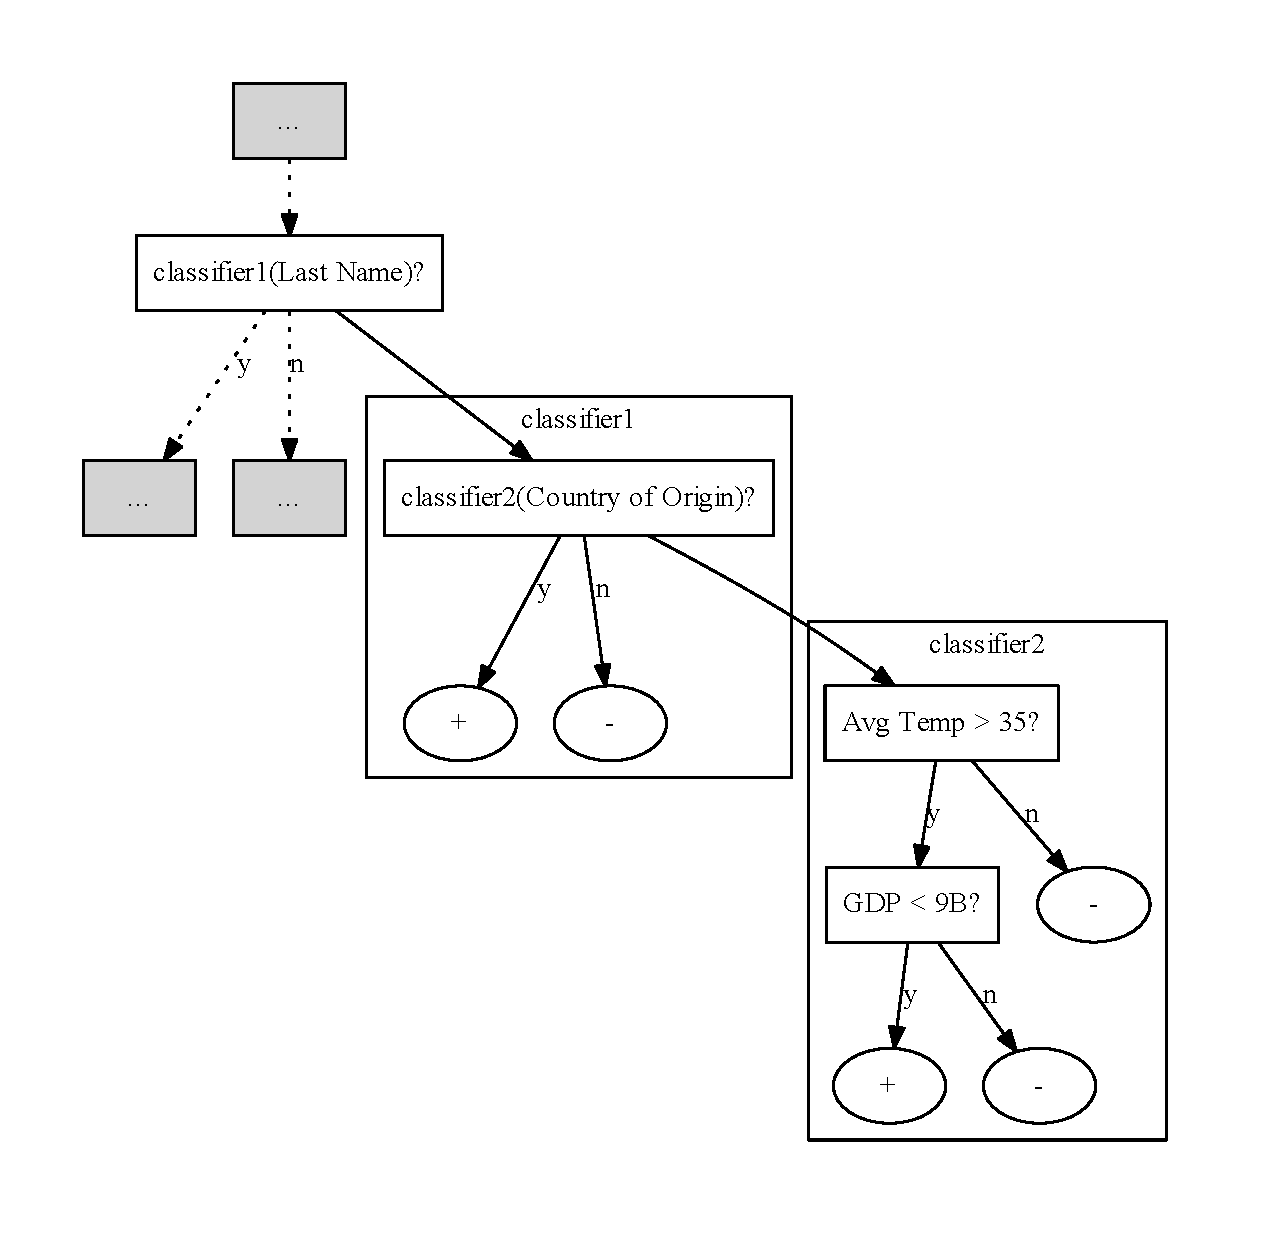
\includegraphics[width=\linewidth]{example.pdf}
	\caption{An example of a generated feature used in a decision tree classifier. Note that a classifier (which is created using relational data) is called on the value of a feature.}
	\label{fig:example}
\end{figure}


%%%%%%%%%%%%%%%%%%%%%%%%%%%%%%%%%%%%%%%%%%%%%%%%%%%%%%%%%%
\section{Background} \label{background}
%%%%%%%%%%%%%%%%%%%%%%%%%%%%%%%%%%%%%%%%%%%%%%%%%%%%%%%%%%

One of the earliest methods of utilizing relational information, officially defined by \citet{muggleton1991inductive} and used even before then in the well-known FOIL algorithm \citep{quinlan1990learning}, is \emph{Inductive Logic Programming(ILP)}. This approach induces a set of first-order formulae
that define a good separation of the given training set. Originally, ILP methods searched the space of first-order formulae to find the appropriate classifier.
Following this work, Relational Learning - techniques designed to utilize relational databases, have become increasingly prevalent. One such technique is that of View Learning \citep{davis2005view}, which generated new tables from existing ones, effectively performing feature generation for relational methods.

One major attempt at adding relational knowledge to traditional induction algorithms was \emph{propositionalization} \citep{kramer2000bottom}: Since we wish to allow the use of first-order predicates in propositional methods, we create possible (non recursive) first-order predicates in a process known as refinement search \citep{van1998completeness}.
We define a graph of possible first-order formulae by selecting an initial relation and allowing one of two possible refinement operators: The first operator is binding a single variable in the formula by assigning a constant value to it, and the second is binding a single variable using another relation.

These operators define a search space. For each formula, we can ask whether a given object satisfies it, giving us a binary query for the data. We often prefer to only use formulae with one unbound variable, as it simplifies the satisfaction check.
It is important to note that each application of refinement operators yields a formula that is subsumed by the parent, meaning that any object satisfying the child formula will also satisfy its parent.

A major setback of this process is that it generates an impractically large number of features, most of which irrelevant.  To this end, \emph{upgrade} methods such as ICL \citep{van2001upgrade} were suggested, where instead of creating predicates a-priori, we do so during the training phase, allowing us to avoid searching non-promising refinements.

As a continuation to this trend, \citet{popescul200716} suggest SGLR, an upgrade method which allows the generation of nominal attributes by using aggregation operators. Essentially, instead of simply checking whether a first-order predicate is satisfied, we perform aggregation over all objects which satisfy it. In addition, SGRL offers an initial insight into the issue of improving the search process by using Akaike's information criteria (AIC, see \citet{burnham2002model}) to select features based on a combination of complexity and predictive power. 

%In the case where this external knowledge is organized as a set of relations between entities, several methods can be used. One such method is using \emph{Inductive Logic Programming} \citep{muggleton1991inductive} to generate features, in a process referred to as \emph{upgrading} \citep{van2001upgrade}. This is demonstrated through the ICL algorithm, which uses a refinement graph to search for logical formulae which serve as features. The SGLR algorithm \citep{popescul200716} extends this idea to numerical features, generated using aggregation-based techniques, and then utilizes regression for inference.

%Newer advances in the relational approach can be seen in the field of \emph{Statistical Relational Learning} \citep{blockeel2013statistical, nath2014learning} as well as the task of \emph{Collective Classification} \citep{laorden2012collective, kajdanowicz2013collective}. The general field of Statistical Relational Learning (and reasoning) deals in tasks where there is a complex, relational structure within the domain. Common tasks in the field are: Collective classification, link prediction and entity resolution between datasets. Of these, the most relevant to our domain is the task of collective classification, where relational information is used to infer labels of objects based on related objects. However, this relational information is not used for feature generation, but as a way to link objects within the target domain.

%should possibly be moved to related work
Recently, there has been a strong trend of utilizing \emph{Deep Learning} \citep{lecun1998gradient, bengio2009learning} as a feature generation technique. These methods essentially form combinations and transformations on pre-defined features in a semi-supervised manner, thus yielding new, more predictive features.
There are many good examples of this, such as the ones presented in \citet{plotz2011feature} and \citet{kim2013deep}.

An interesting domain can be found in a well-known and well-explored task within the field of Natural Language Processing (NLP): the task of text classification.
this task involves assigning categories or labels to documents, based on their content. The potential labels/categories are given in advance, and we have a collection of labeled documents to use as a training set. This task has many practical applications, such as spam filtering, sentiment analysis and topic identification.

Until recent years, text classification systems represented text almost exclusively as a \emph{Bag of Words}, thus creating a vector space representation \citep{Wu:1981:CST:1013228.511759, salton1983introduction}. While this method offered simplicity, it had inherent limitations in terms of representation power.

A major breakthrough came in the form of the \emph{explicit sematic analysis} \citep{gabrilovich2009wikipedia} method, which used semantic concepts extracted from knowledge sources such as Wikipedia as features. This technique allowed for a richer representation of the text, and has shown improvement over the Bag-of-Words representation for the task of text classification, especially in shorter texts.

%this one is pointless, right?
%The goal of our work is to utilize Linked Data as a knowledge source for automatically generating features based on meaningful semantic concepts, thus improving existing machine learning algorithms. We intend to do so in a supervised manner to allow a better guided search over candidate features, based on a combination of complexity and predictive power. We will place focus on the domain of text classification as a natural application of our approach.

%%%%%%%%%%%%%%%%%%%%%%%%%%%%%%%%%%%%%%%%%%%%%%%%%%%%%%%%%%
\section{Generating Features through Recursive Induction}
%%%%%%%%%%%%%%%%%%%%%%%%%%%%%%%%%%%%%%%%%%%%%%%%%%%%%%%%%%

Let $O$ be a set of objects. Let $Y=\{0,1\}$ be a set of labels (we assume binary labels for ease of discussion). Let $S=\{(o_{1},y_{1}),\ldots,(o_{m},y_{m})\}$ be a set of labeled examples such that $o_{i}\in O, y_{i}\in Y$. Let $F=\{f_{1},\ldots,f_{n}\}$ be a \emph{feature map}, a set of \emph{feature functions} $f_{i}:O\rightarrow Dom_{i}$.  This definition implies a training set represented by feature vectors: $\{ (\langle f_1(o_i),\ldots,f_n(o_i)\rangle, y_i) | (o_i,y_i) \in S\}$.

Given a set of relations $\bar{R}=\{R_{1},\ldots,R_{t}\}$ with arity of $n_{j}$ ($j=1\ldots k$), we can assume \text{w.l.o.g} that the first argument is a key. For each relation $R_{j}$ we define $n_{j}-1$ new binary relations where each of the first elements is the key and the second one is another column.
Let ${\cal R}=\{R_{1},\ldots,R_{k}\}$ be such set of binary relations, where $R_{i}$ is defined over $K_{i}\times D_{i}$. These relations can thus be seen as functions $R_{i}: K_{i}\rightarrow D_{i}$.

\begin{defn}
	A \emph{supervised feature generation algorithm} $A$ using relations is an algorithm that given $\langle S,F,{\cal R} \rangle$, creates a new feature map $F_{\cal R}=\{f'_{1},\ldots,f'_{l}\}$.
\end{defn}

We would like the new hypothesis space, defined over $F_{\cal R}$, to be one that is both rich enough to provide hypotheses with a lower loss than those in the original space, as well as simple enough that the learning algorithm used will be able to find such good hypotheses given training data.
%We would also like there to be connections between $F$ and ${\cal R}$, meaning some of the feature values of features in $F$ (when applied to objects in $S$) also exist within relations in $\cal R$.

\subsection{Generating a feature} \label{algorithm_section}

Given an original feature $f_{i}$ with domain $Dom_i$, our algorithm will formulate a new learning task trying to separate values in $Dom_i$ appearing in positive examples of the original learning task from those appearing in negative ones.  The result of the new learning task will be a classifier
$h_{i}:Dom_{i}\rightarrow \{0,1\}$ that can label feature values of $f_{i}$. We can then define a new binary feature $f'_{i}(x)=h_{i}(f_{i}(x))$.
We name this algorithm \emph{RI-Tree}, as it performs recursive induction and makes use of a decision tree to generate features in local contexts (For pseudo-code, see appendix \ref{app:2}).

In order to explain how we create such $h_{i}$, let us consider a single step of the feature generation algorithm.
Given a feature $f_{i}$, we define the set of all its value in the training set $S$ as $v_i(S) = \{v | (o,y) \in S, f_{i}(o)=v\}$. In the intro example, for instance, $v_i(S)$ will be the set of all last names of patients.
We now formulate a new learning problem with the new training set
$\hat{S_i} = \{ (v, label(v)) | v \in v_i(S) \}$.
The labelling function can be, for example, defined as
the majority label: $label(v)=majority(\{y_k| \left(o_k,y_k \right) \in S, f_{i}(o_k)=v\})$.

To define a feature map over the new training set $\hat{S}$, we look for all relations in $\cal R$ where the domain of the key argument contains $v_i$:
${\cal G}(S,{\cal R}) = \left\{ r \in {\cal R} | v_i(S) \subseteq \{x_1 | (x_1,x_2) \in r\}\right\}$. In the intro example, one such $r$ can be a relation mapping last names to countries of origin. We then use ${\cal G}$ as a feature map for $\hat{S_i}$.
Solving this new learning problem on $\hat{S_i}, {\cal G}(S,{\cal R})$ yields our classifier $h_{i}$.
Note that during the process of learning $h_{i}$, we can once again call the feature generation procedure to generate useful features for the \emph{new} task, hence the recursive aspect of the process. We can see this in the intro example, wherein we construct a second-level problem on countries of origin to correctly identify the appropriate conditions that signify high risk countries.

When performing feature generation, we often wish to evaluate the predictive power of generated features. When such evaluation is done in the context of the entire dataset, it is possible to lose the unique benefit of a potentially powerful feature. To address this phenomenon, we decided to perform and evaluate our feature generation algorithm within local contexts through the use of a decision tree. It is important to note, however, that the features generated in this process can be used for any induction algorithm, not necessarily decision tree induction algorithms.
Using decision trees has several advantages: 
\begin{itemize}
	\item We gain an innate way to evaluate and filter generated features: A feature generated in a node will be added to the final result only if it achieves a higher information-gain than the most informative existing feature. %We further require that the features achieve a significantly better $\chi^2$ score on the training examples.->this part is not accurate!!!
	\item Since we repeat this process within inner nodes of the tree, we allow for the discovery of locally relevant relationships which may be difficult to pick up when looking at the entirety of the data. We use pre-pruning based on minimal leaf size to avoid creating features which are poorly supported by actual training data.
	\item Since a decision tree classifier tests features one at a time, we can easily isolate the impact of a specific generated feature.
	\item Since we use generated features in the constructed tree, we can ensure that features generated afterwards within the tree will be largely orthogonal to it, thus ensuring variety in the generated features. %is this accurate?
	\item Decision trees are relatively interpretable, which leads to features which are easier to understand.
\end{itemize}
Naturally, we use decision trees as the classifiers for the newly constructed learning problems as well, allowing us to easily repeat the process recursively. This also means we can construct features which mix multiple levels of abstraction by having some of the nodes within the tree be constructed features and others be regular ones. In the into example, we could decide that if the country of origin appropriate for a person's last name is a country at risk, we must still ask whether the person's last name is their maiden name, as the constructed feature would otherwise yield a false positive.

Finally, the features generated during the decision tree training procedure are collected and returned for use as general, black-box features which can be used along with any induction algorithm.

\subsection{Analysis}

%I honestly have no idea where I'm going with these, so mby...
%Due to the nature of the feature generation method, the generated features are decision trees. These features capture a subset of feature values linked in the semantic domain through a shared relational chain 

We can look at the recursive feature generation process as a search problem over the DAG of possible domains:
\begin{defn} Domain:\\%defined recursivly. add that we can do ANY transform G using S,R,F
	$S$ is a domain.
	If $\bar{S}$ is a domain, then for any function $G_{\bar{F},\bar{R}}: O\rightarrow Dom_i$, $\bar{S'}=\{(v_i,label(v_i)|(o,y)\in \bar{S}, v_i=G_{\bar{F},\bar{R}}(o)\}$ is also a domain.
\end{defn}
The result bears some similarity to the process of searching over a refinement graph in the field of Relational Learning.
In order for this search space to be a acyclic, we must take care to avoid cycles by refusing to return to already explored domains. This also makes sense from an algorithmic perspective, as there is no new information to be gained by this.

The aforementioned feature generation approach offers some unique contributions:
\begin{itemize}
	\item By moving our domain space when constructing a new problem, we essentially look at the problem from another perspective, which allows for the discovery of complex relationships.
	\item The process of re-labeling allows noise reduction and emphasizes more general trends within the data that may be harder to otherwise notice.
	\item We can exploit the power of existing, well-developed learning algorithms when we create a classifier, and possibly use different ones as we take recursive steps.
	\item By using a decision tree, we can find locally good features, which often translate to globally good features.
\end{itemize}


\subsection{Applications for Text Categorization}
In order to apply our feature generation technique to the domain of text categorization, we make the standard assumption that our basic features are the words that appear in the texts. We can therefore take words which also exist as entities within the relational database as feature values $v_i$ for the sake of our approach.
The resulting features will locate sets of words which are connected in the relational domain. This allows us to better generalize compared to the standard bag-of-words method, and find potentially complex semantic relationships, especially when using Semantic Linked Data as our relational database.

An important side effect of this usage is that, since each label in the semantic data defines a relation and texts may contain words from different contexts, there are often multiple relations which apply and thus ${\cal G}(S,{\cal R})$ is often large. For example, a text referring to William Shakespeare's play of "Hamlet" may connect to relations on people (for William Shakespeare himself), on theatre plays (for "Hamlet"), and possibly locations (for the country of Denmark, where the play is set).
In order to make the process more computationally tractable, especially if it is performed recursively, we uniformly choose a sub-sample of ${\cal G}(S,{\cal R})$ for which we construct new learning problems.

A second relevant difference to note is that generated feature may be non-applicable to a specific object, as it may be the case that none of the words within the text appear in a given relation (or, in fact, within the knowledge base at large). Therefore, we decided to use a third value for cases where the generated feature does not apply.

%this entire section!
\section{Empirical Evaluation}
In this section, we discuss our experimental methodology and display our main results.
\subsection{Methodology}
We have evaluated our method on the TechTC-100 collection \citep{gabrilovich2004text}, a collection of 100 different datasets containing binary text categorization problems of varying difficulty extracted from the Open Directory Project.

%expand?
As a knowledge base, we used YAGO2 \citep{hoffart2013yago2}, omitting any relations with literal data such as dates or geographic coordinates. This served as a "common knowledge" database. We also made limited use of type information within the database.

We ran our feature generation algorithm for both depth 1, i.e., creating a recursive learning problem for the original problem, as well as depth 2, creating recursive learning problems for the original problem and the first order recursive problem.

We compared the new set of features (our new features combined with standard binary bag-of-words features) to the original binary bag-of-words features at various feature selection levels. We used information gain as the feature selection criterion.
\subsection{Results}
%results, specific examples (qualative analysis), explaining it and so on
Figure \ref{fig:accuracy} shows the average accuracy across all datasets within techTC-100 over various feature selection levels. We show our method for both depths, compared to the non-relational case.  The left graph shows the accuracy using K-Nearest Neighbours \citep{fix1951discriminatory} as our classifier ($K=1$) and the right graph shows the accuracy using SVM \citep{cortes1995support} as our classifier (Linear kernel, $C=100$). Results ran using CART \citep{steinberg2009cart} as a classifier (requiring a consistent tree) yielded similar results in terms of accuracy to those of SVM, albeit with a higher base accuracy level ($0.73 instead of 0.7$).
We see that the one-level application is better than the simple bag-of-words approach, and the two-level application yields a further improvement. This result is far more apparent in SVM based classification, as the impact of a single powerful feature is much clearer compared to a nearest neighbour approach. The two-level application yields a statistically significant improvement $ (p<0.05) $ over the simple bag-of-words approach for multiple feature selection levels. For instance, when taking $20\% $ of the features, we see a statistically significant improvement for both KNN and SVM classification accuracies (using a paired-t-test). 

Figure \ref{fig:accuracy_low} shows the average accuracy across all datasets within techTC-100 over very low feature selection levels. 
We see that in lower feature selection levels the effect diminishes for both classifier types, as some of the generated features are filtered out by the feature selection process. The lowest feature selection level at which we found a statistically significant improvement is $7.5\%$ for SVM, and $15\%$ for KNN.

\begin{figure}[H]
	\centering
	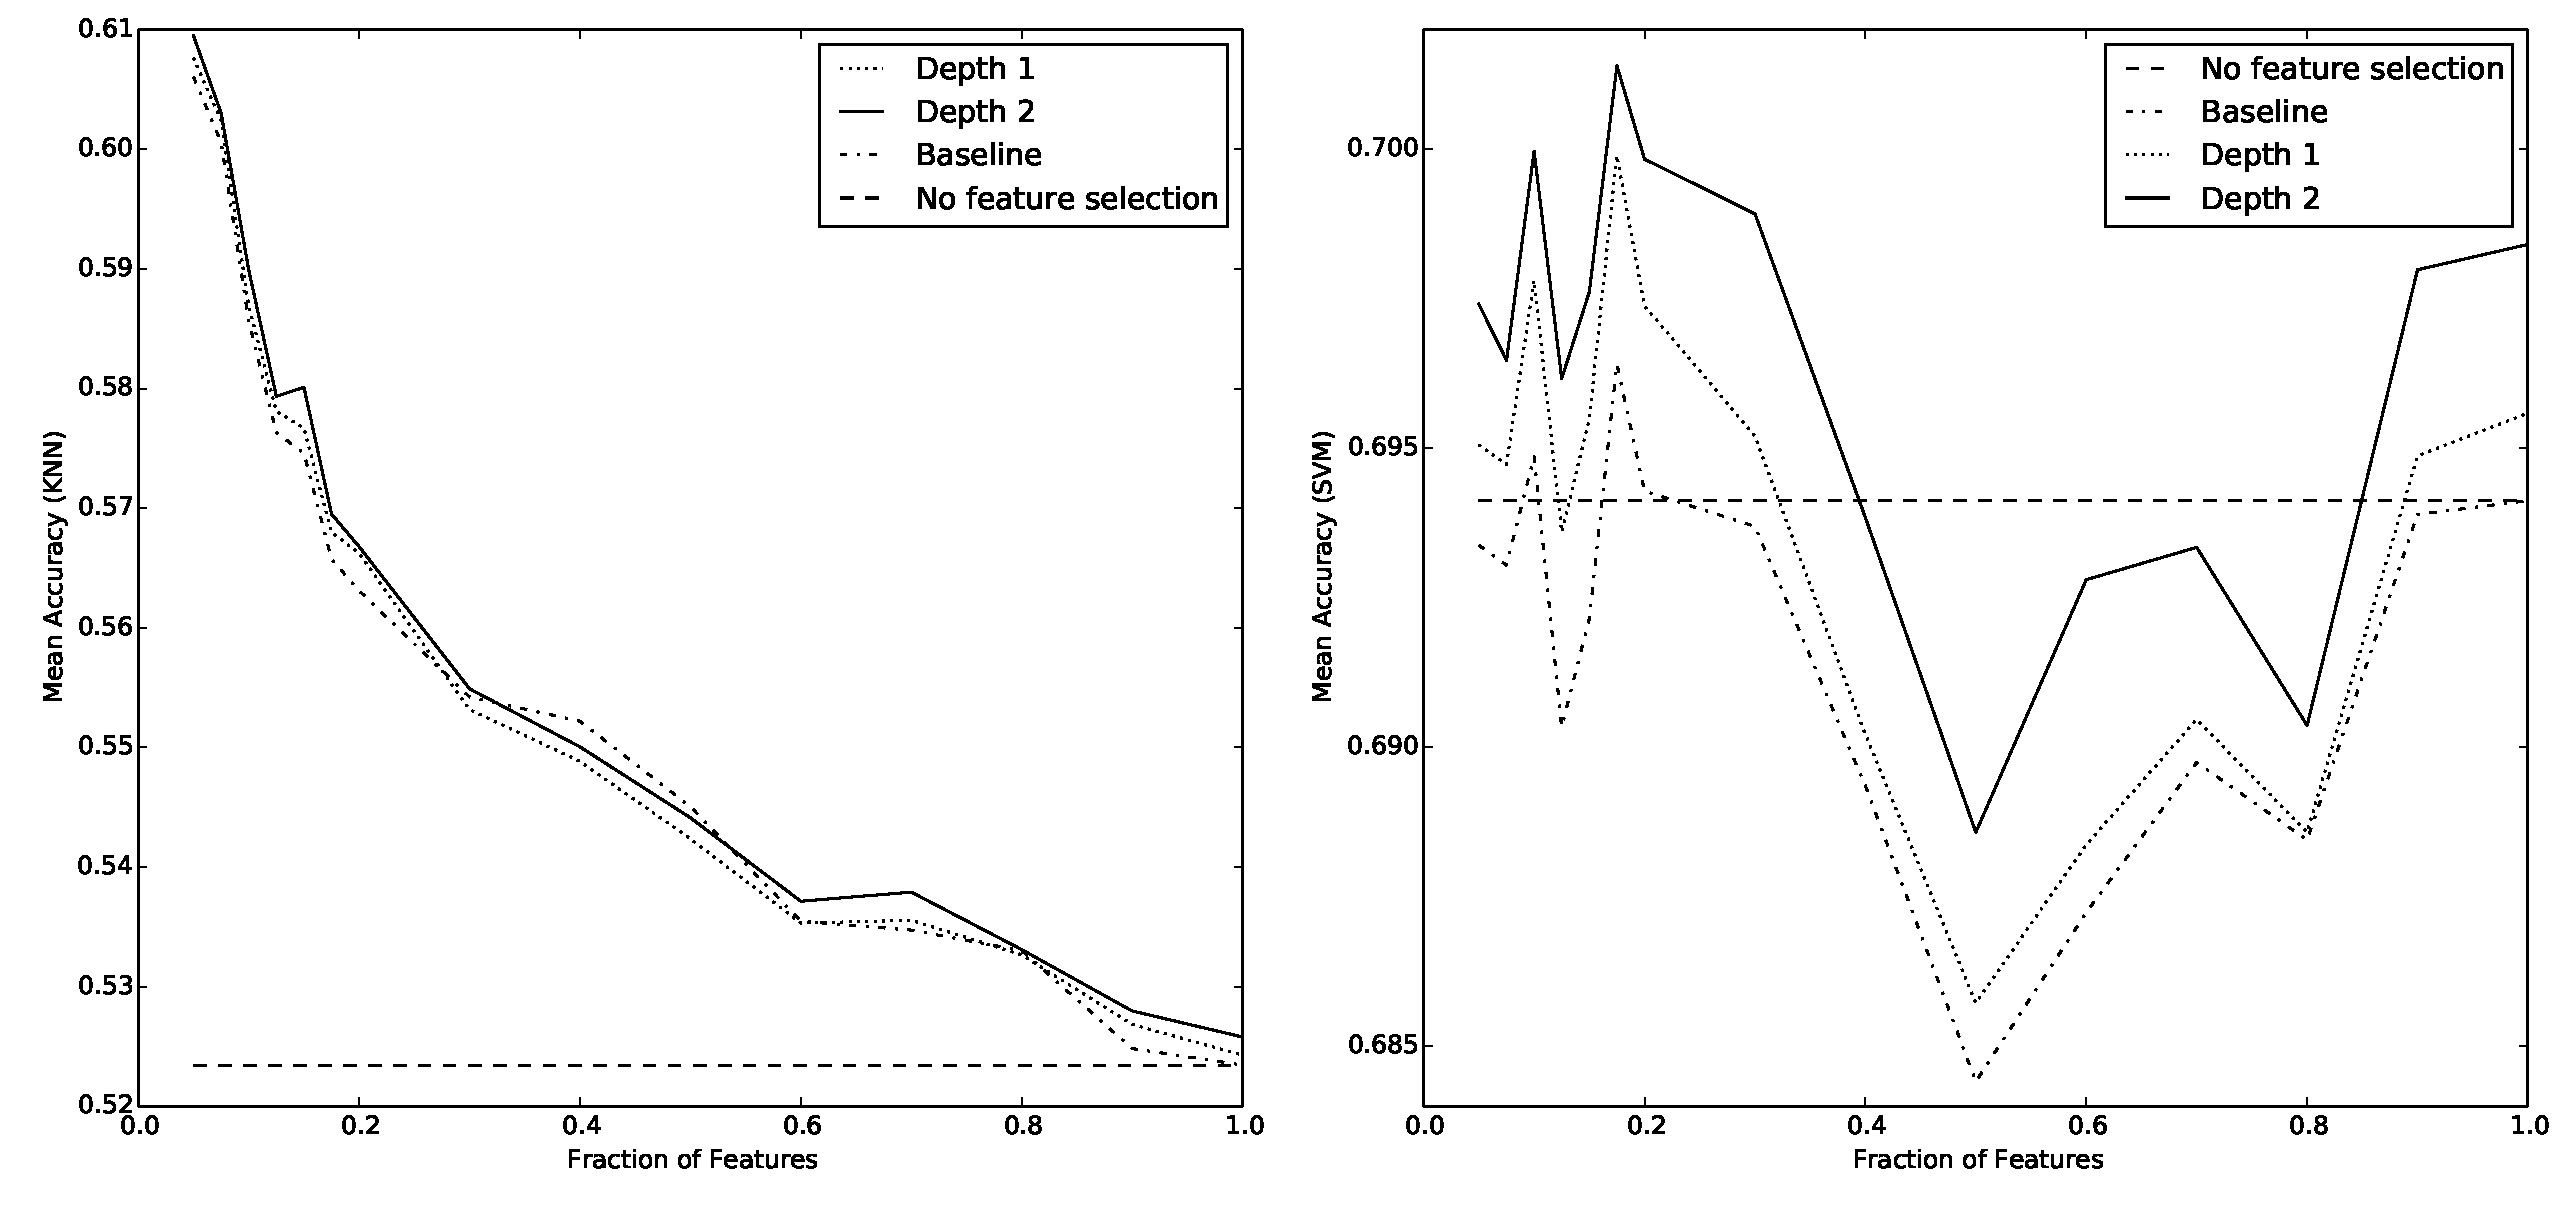
\includegraphics[width=\linewidth]{accuracy.pdf}
	\caption{Average accuracy across all 100 datasets for various feature selection levels. Left side: KNN, Right side: SVM}
	\label{fig:accuracy}
\end{figure}

\begin{figure}[H]
	\centering
	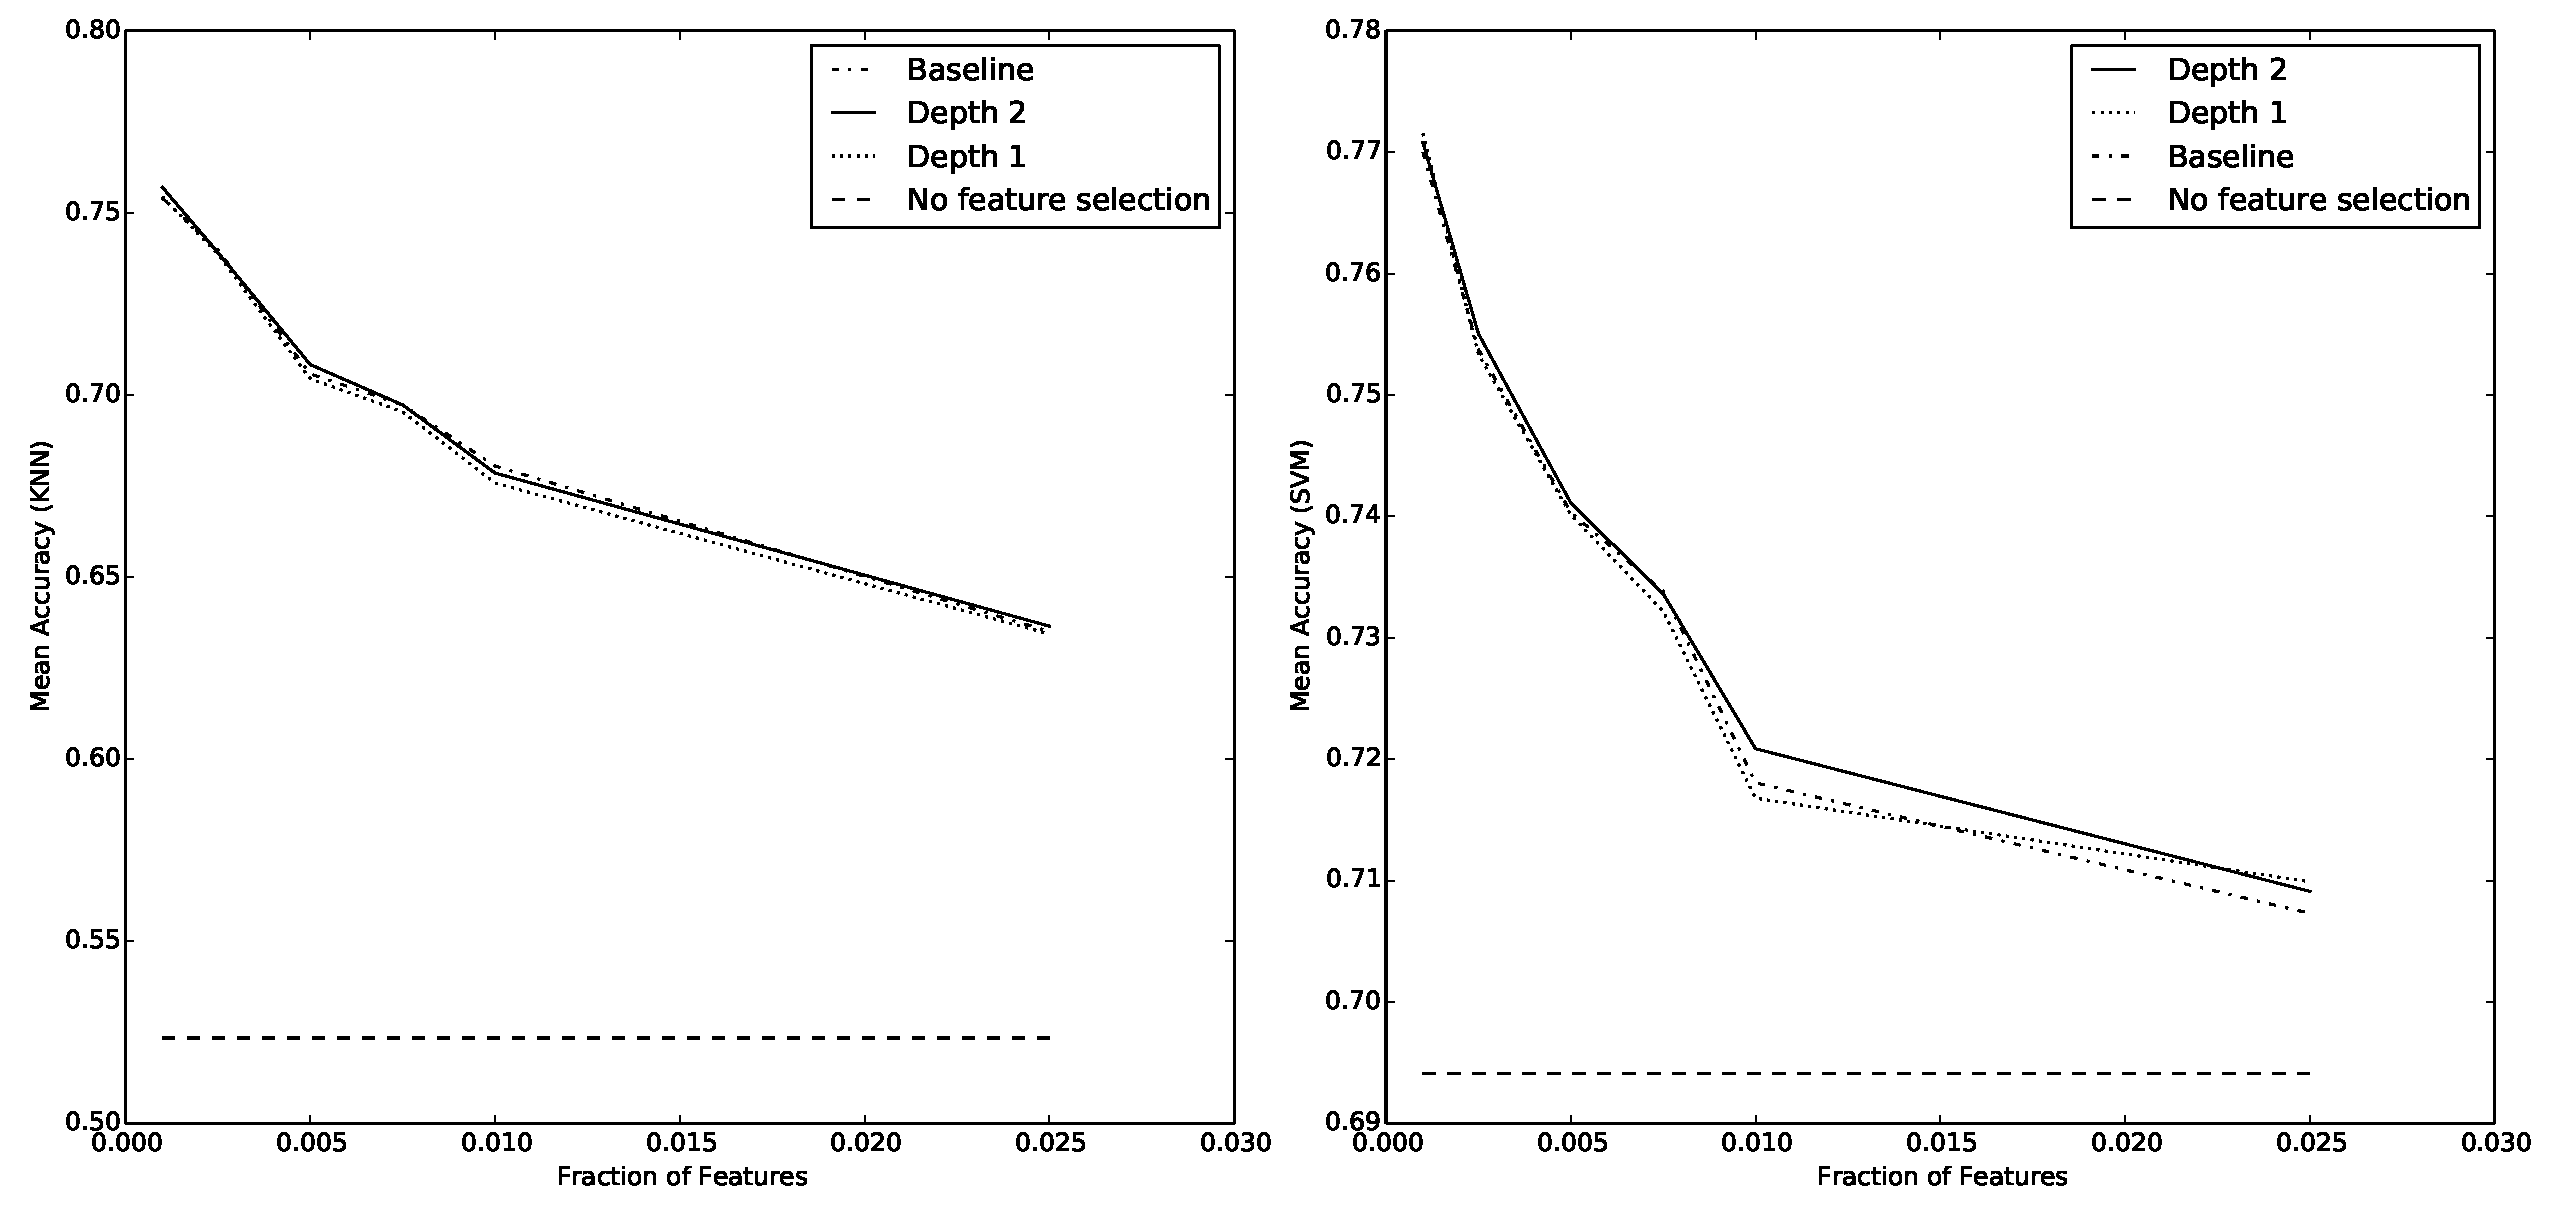
\includegraphics[width=\linewidth]{accuracy_low.pdf}
	\caption{Average accuracy across all 100 datasets for very low feature selection levels. Left side: KNN, Right side: SVM}
	\label{fig:accuracy_low}
\end{figure}

We note that due to the conservative feature generation process, very few features are generated: in nearly half of the datasets within techTC-100, no features are generated at all, and in no single dataset is the number of features greater than five. We also note that all of the generated features arise from local contexts, i.e, when looking at the entire dataset we would have difficulty identifying these features as especially useful. A more careful look at datasets where no features are generated reveals that they tend to have more relations where there are only very few objects in the newly generated problem. Since we only sample some of the possible relations to attempt feature generation, this may be a major factor to the reason no features have been generated.

Figure \ref{fig:ratios} shows the mean ratio between the accuracy of the base approach and the relational approach, and figures \ref{fig:ratios_max} and \ref{fig:ratios_min} show the minimal and maximal ratios accordingly. We note that while the average improvement in accuracy is not large, we can often achieve a $10\%-15\%$ increase, and potentially reach as much as a $30\%$ increase in accuracy for some datasets within TechTC-100. We also note that it is possible to have a decrease in accuracy, but we note that for most cases, especially when using SVM as the classification method, we can limit it to no more than a $10\%$ decrease. Results for CART are once again similar to those of SVM, but with higher variance in both directions.

\begin{figure}[H]
	\centering
	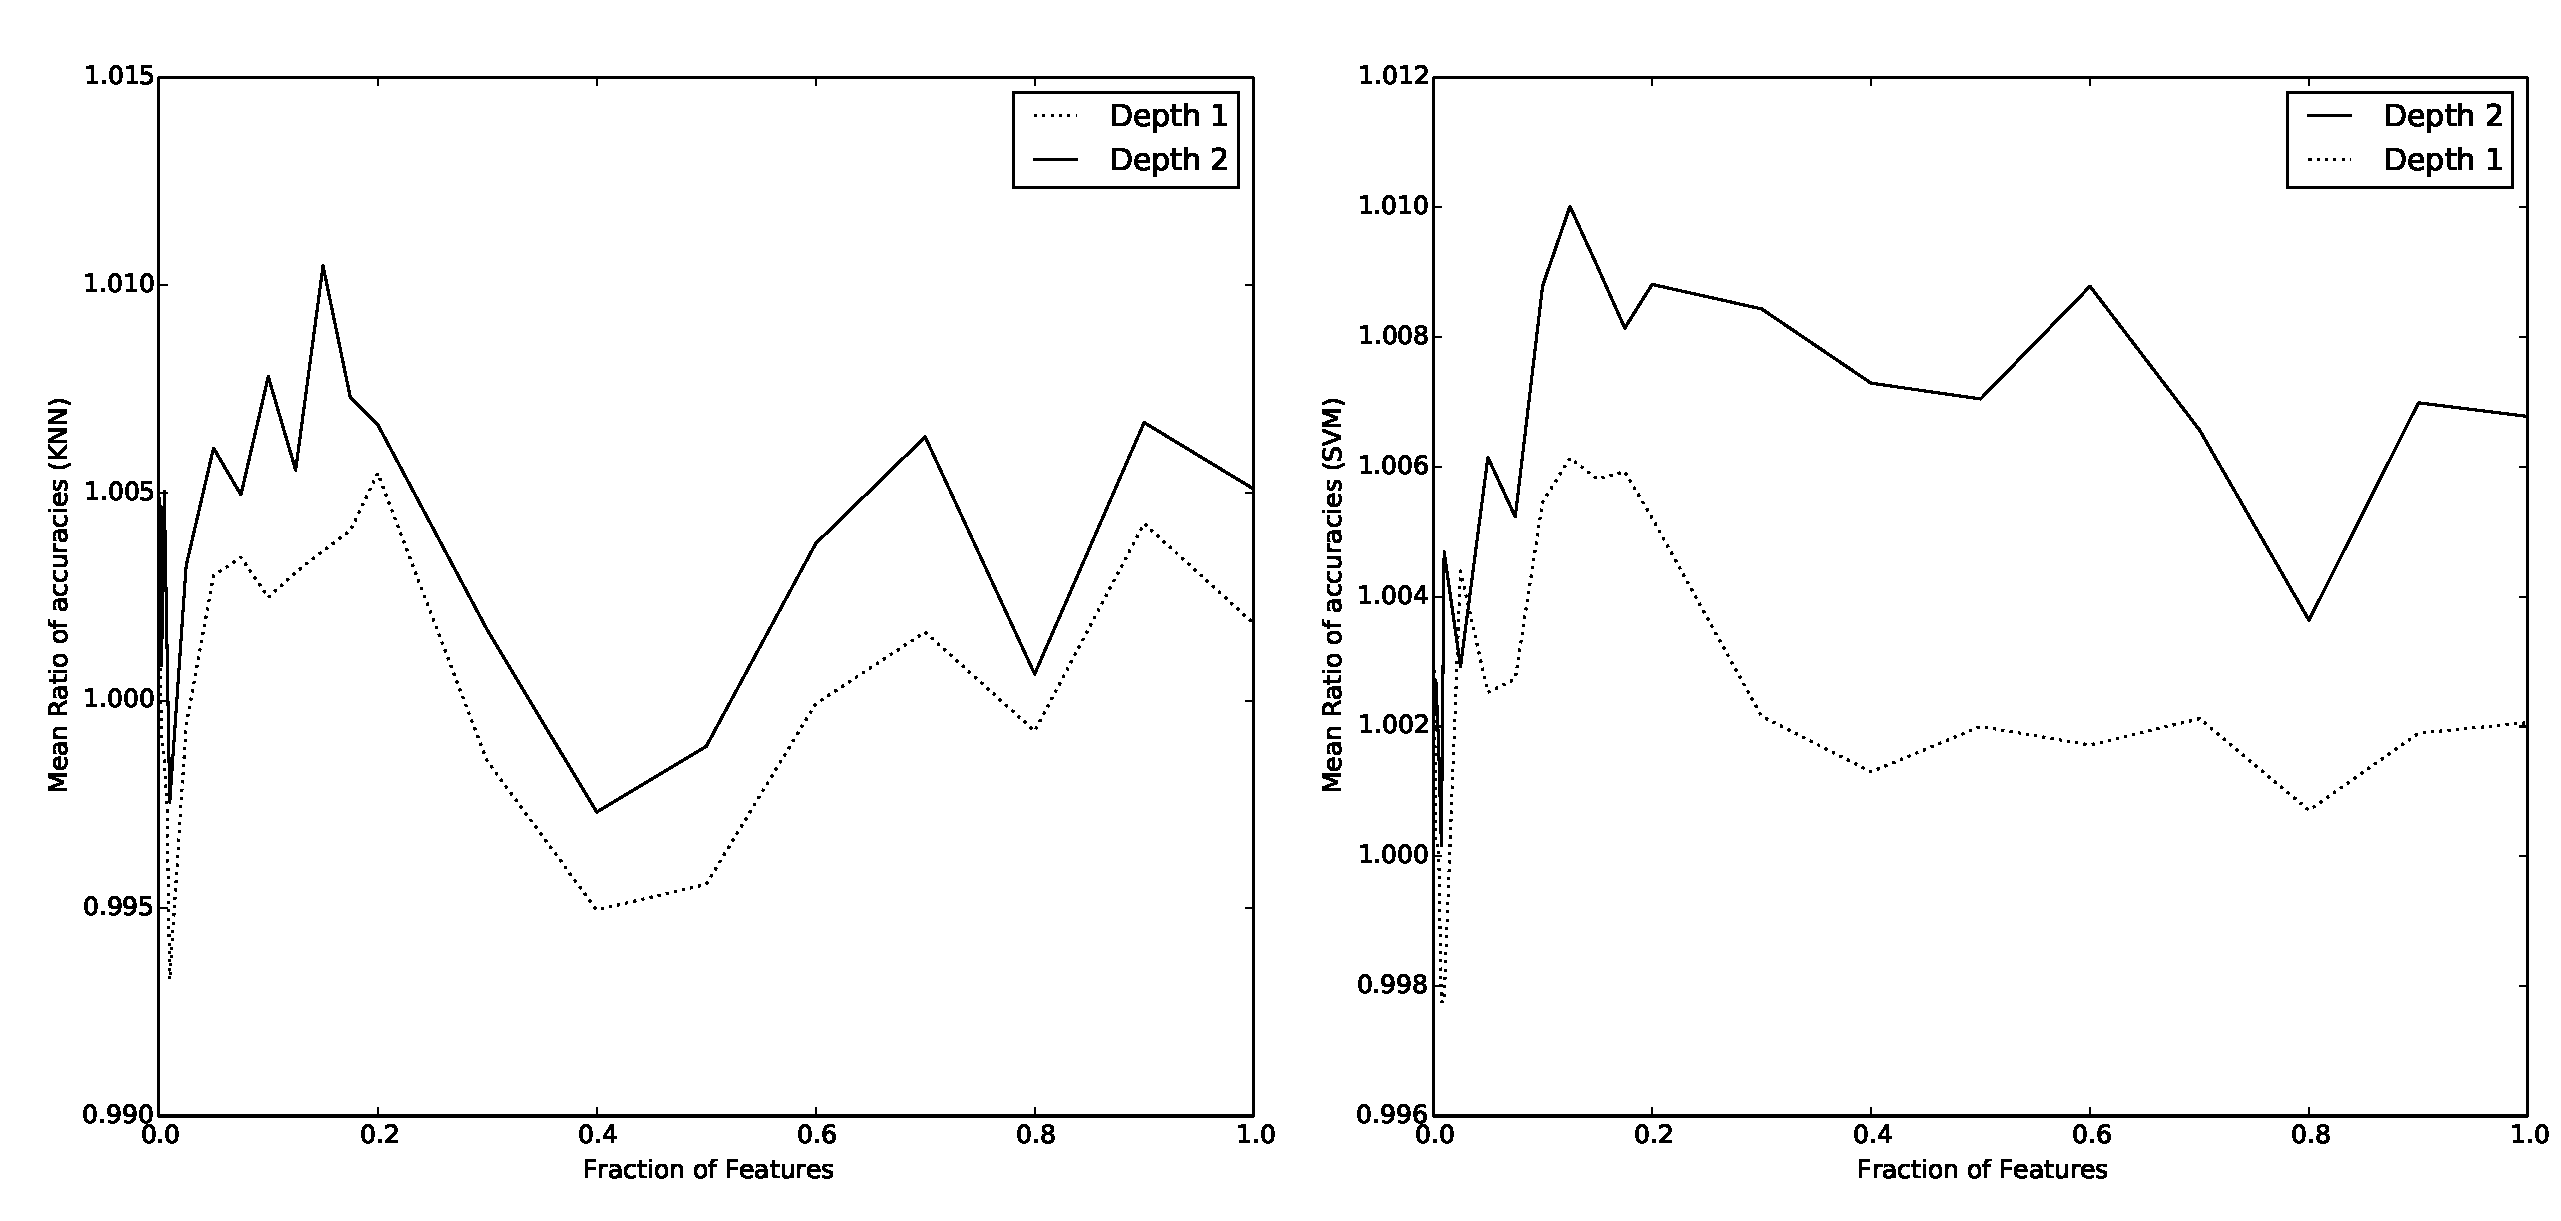
\includegraphics[width=\linewidth]{ratios.pdf}
	\caption{Average accuracy ratio across all 100 datasets for various feature selection levels. Left side: KNN, Right side: SVM}
	\label{fig:ratios}
\end{figure}

\begin{figure}[H]
	\centering
	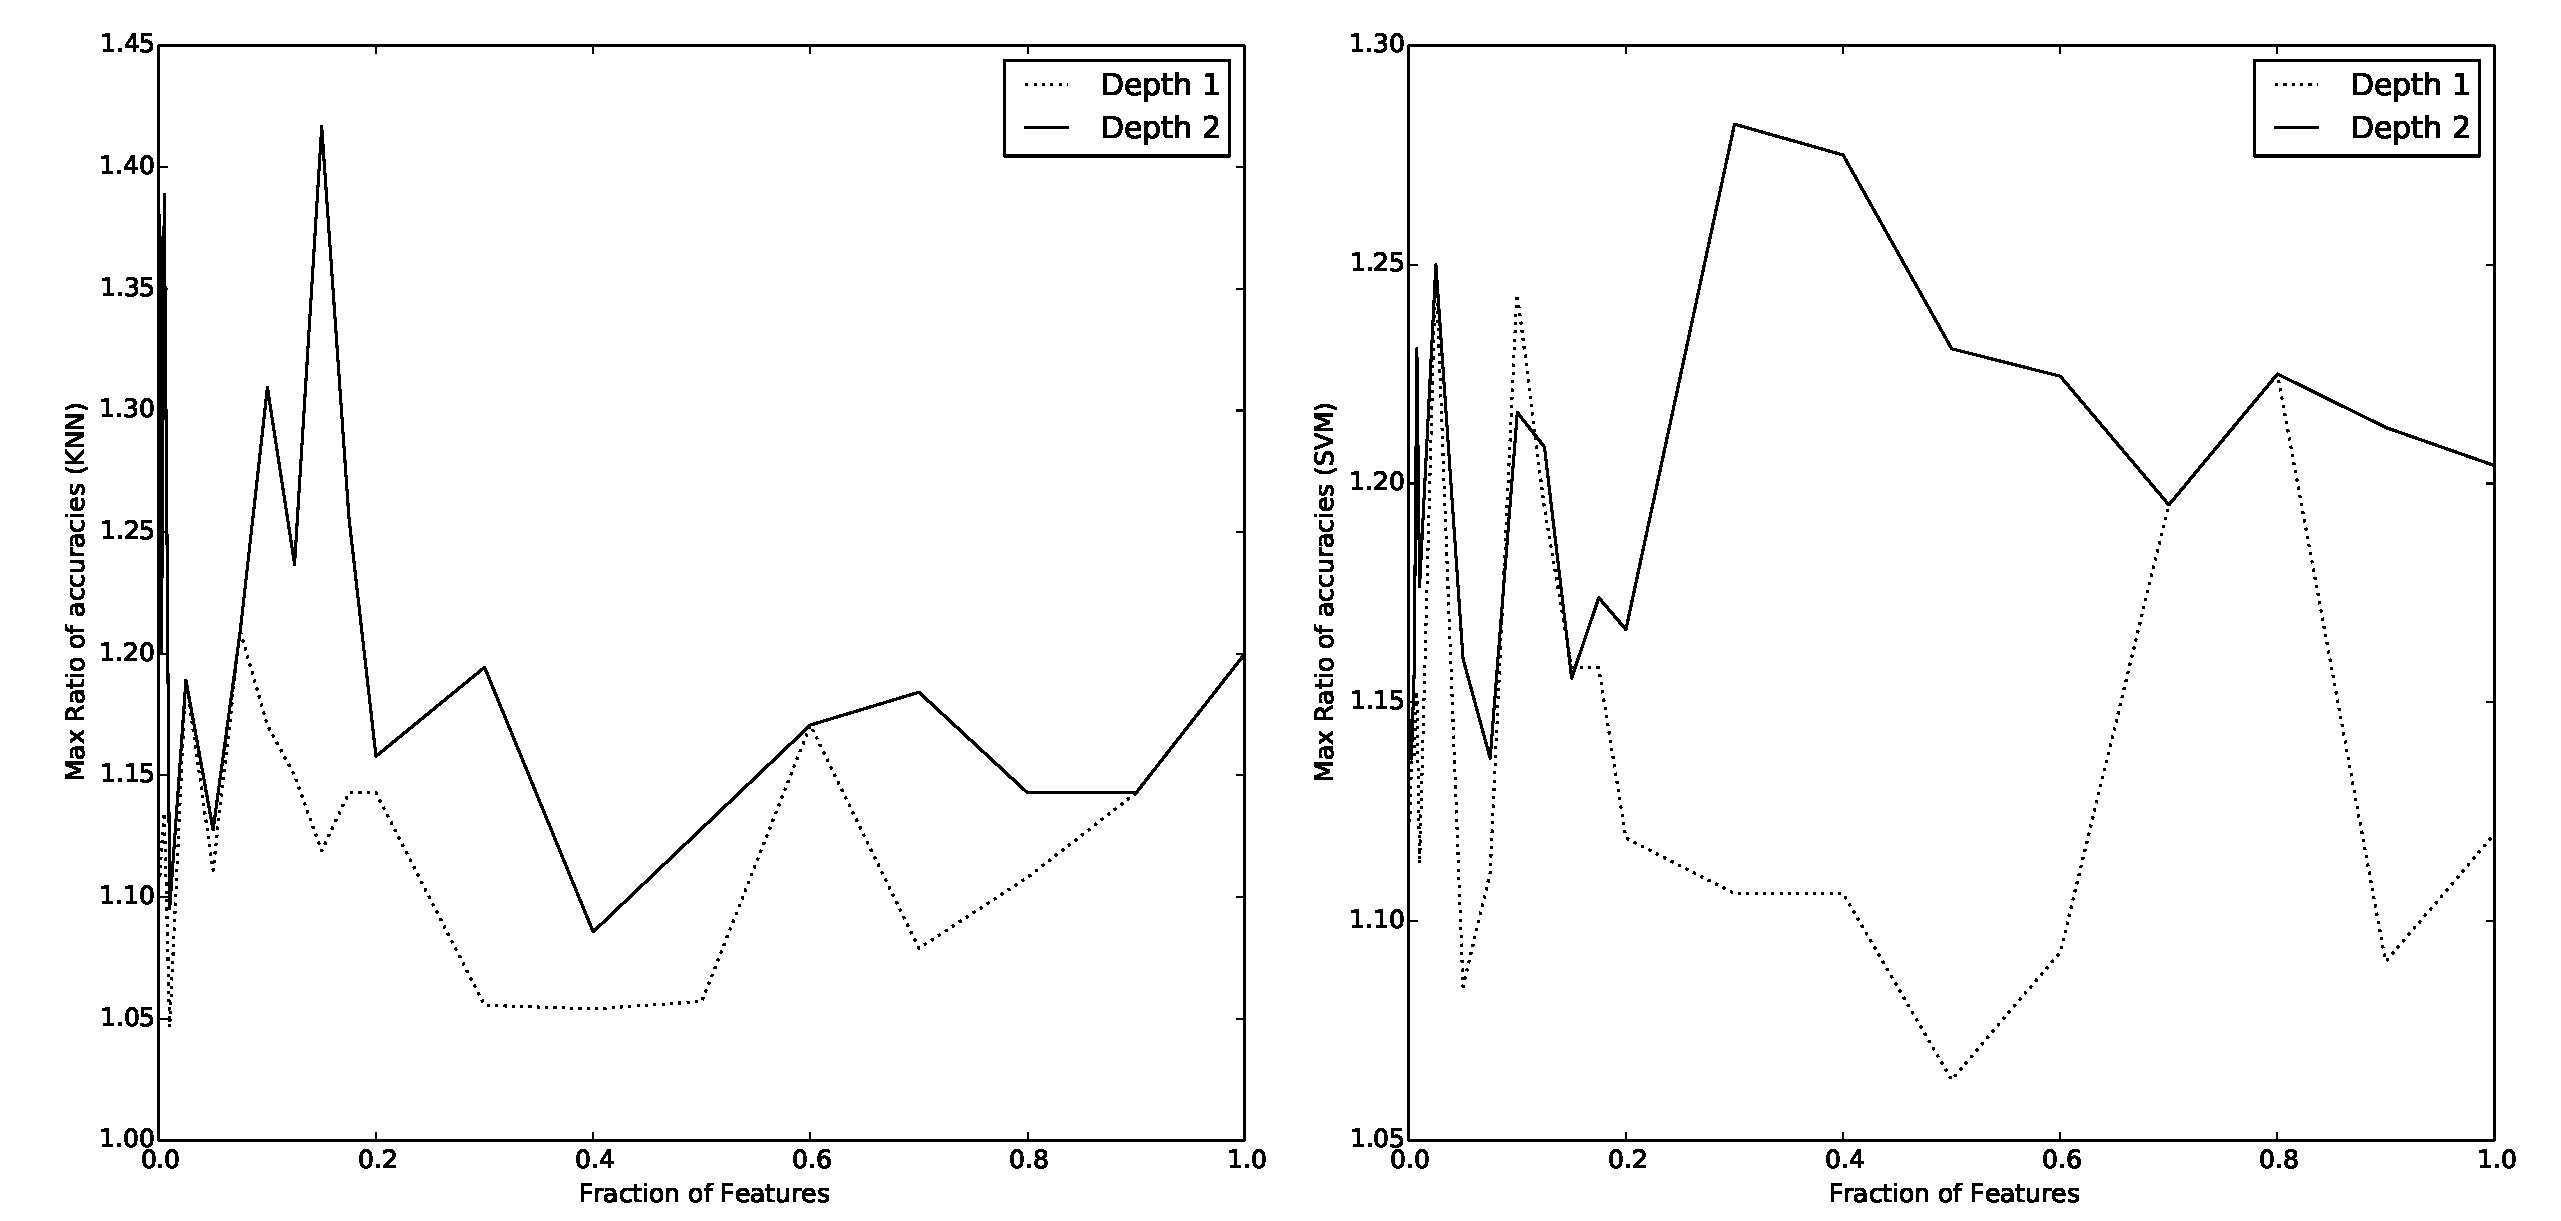
\includegraphics[width=\linewidth]{ratios_max.pdf}
	\caption{Maximum accuracy ratio across all 100 datasets for various feature selection levels. Left side: KNN, Right side: SVM}
	\label{fig:ratios_max}
\end{figure}

\begin{figure}[H]
	\centering
	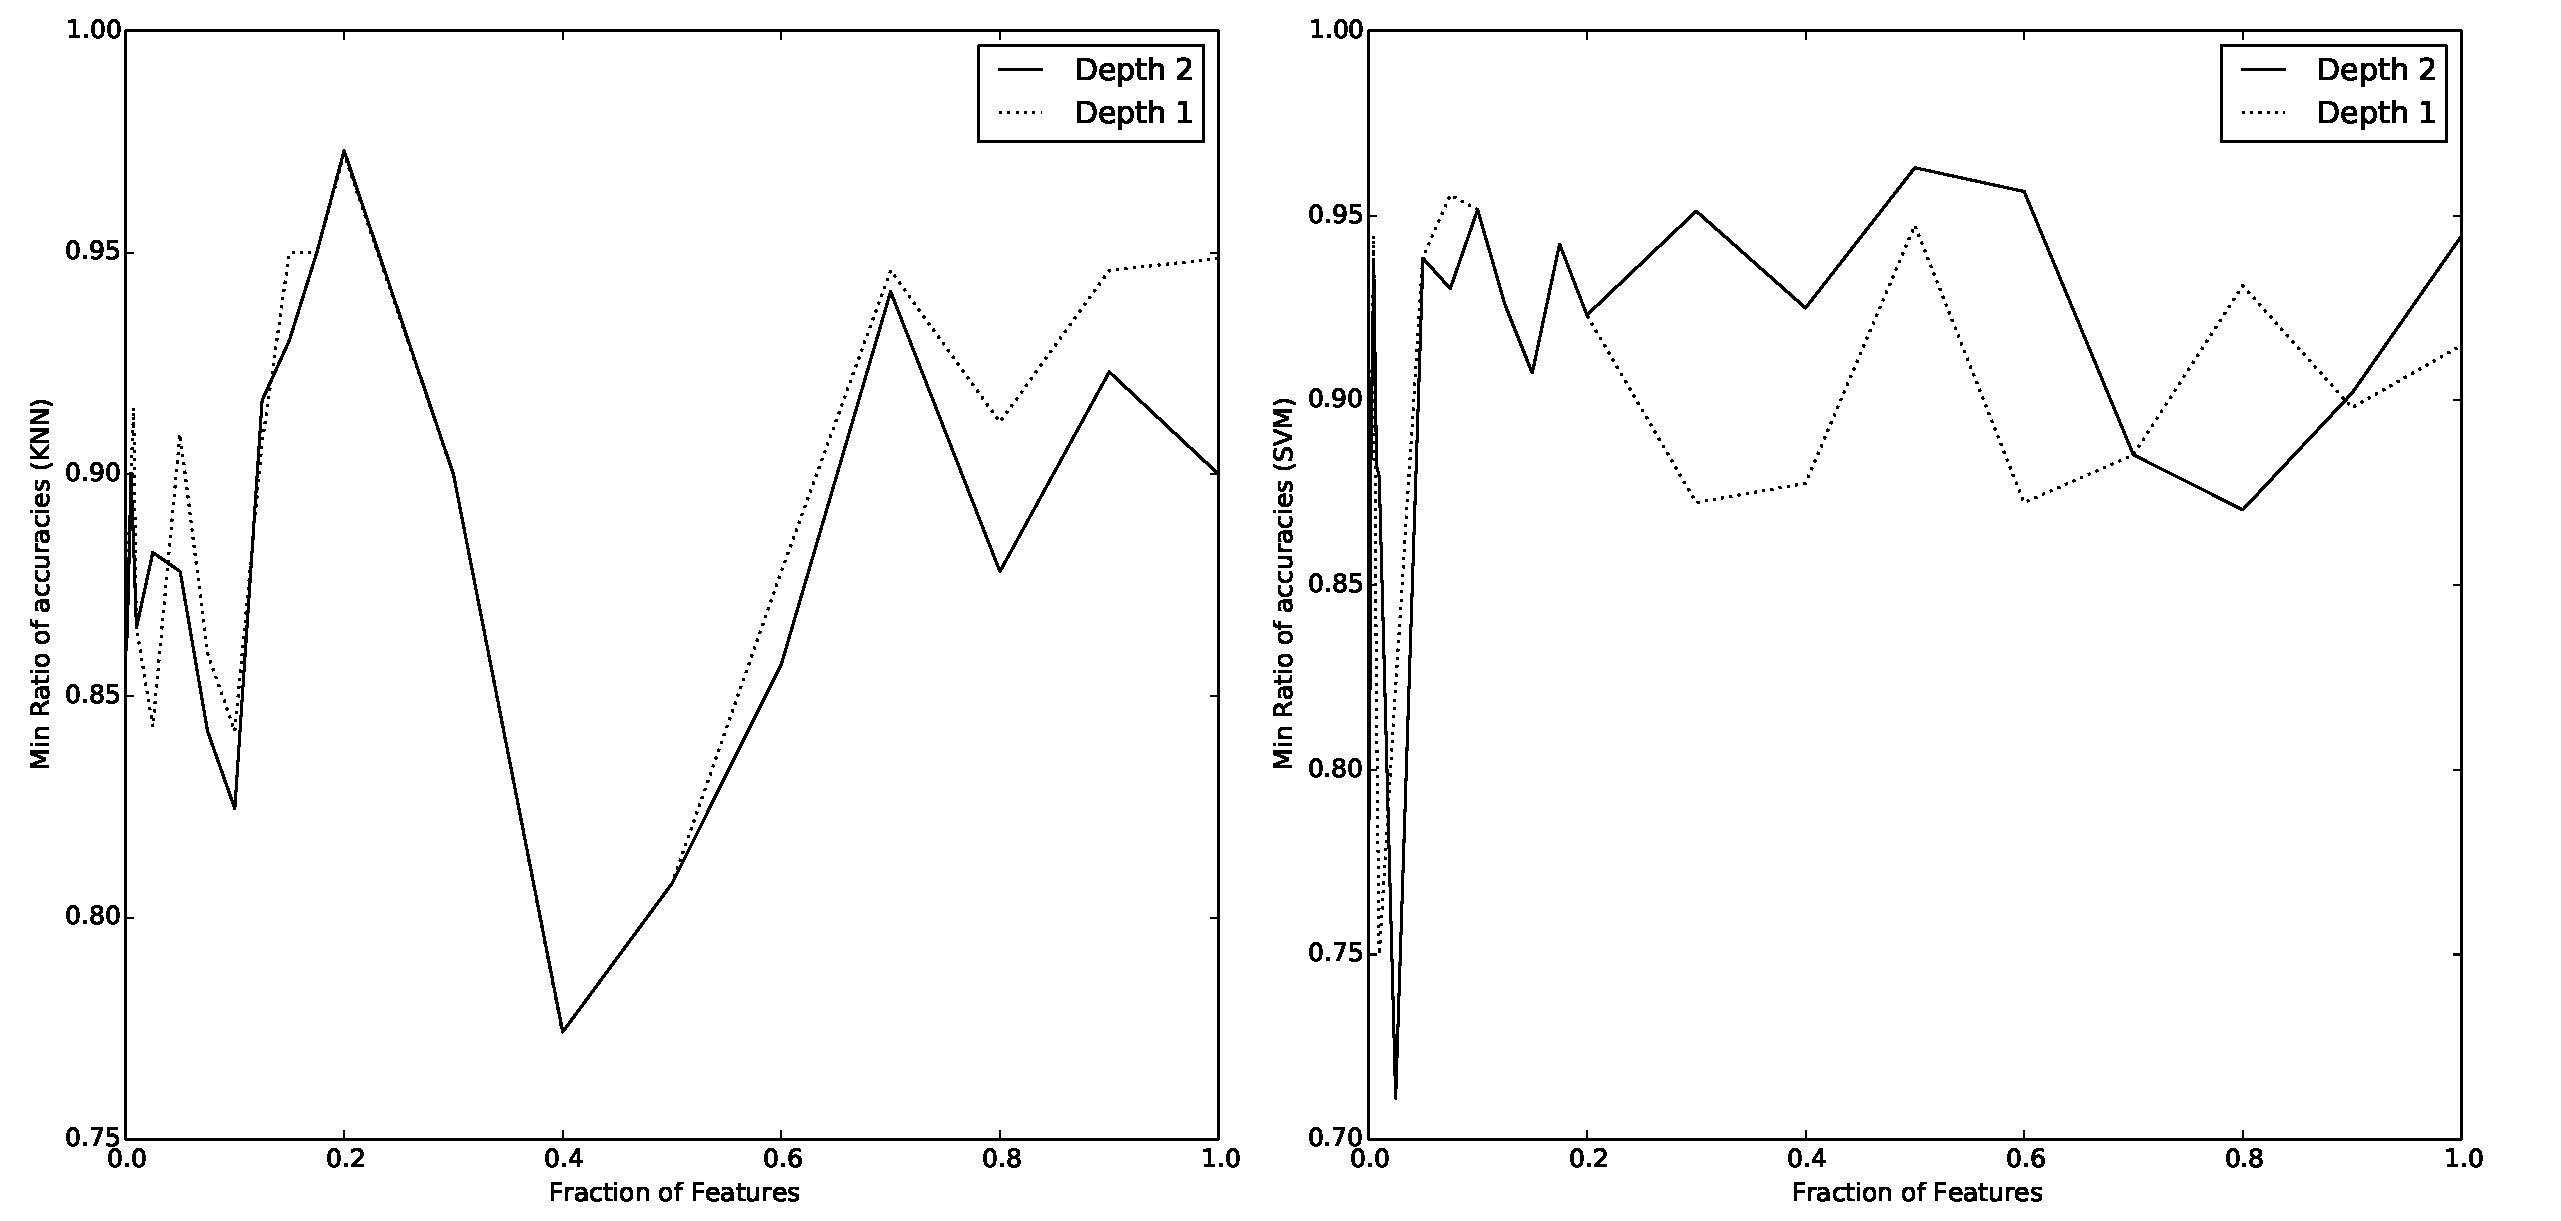
\includegraphics[width=\linewidth]{ratios_min.pdf}
	\caption{Minimum accuracy ratio across all 100 datasets for various feature selection levels. Left side: KNN, Right side: SVM}
	\label{fig:ratios_min}
\end{figure}


\subsection{Qualitative Analysis}
In order to better understand the contribution of these features, let us look at several of them to try and better understand them. Figure \ref{fig:tree1} shows one of the features generated for single level feature generation. We can see %do this!!!

%more stuff

\section{Conclusions}
%finishing up and summary
We presented a novel new approach to feature generation using semantic linked data, based on constructing and solving new learning problems in the semantic domain. While we focused on applying this approach to text categorization problems, it is important to note that it is applicable to any classification problem where feature values are categorical and have semantic meanings, such as drug names, cities and so on. While there is no simple way to generalize this approach to numeric features, we believe there are numerous domains where feature values do have semantic meaning, even excluding text categorization problems.

While our approach only generates binary features, aggregation based techniques such as those used in SGLR apply here as well. A major source for potential improvement is the subject of matching values to semantic objects. Given the major advances in the field of Wikification \citep{bunescu2006using, cheng2013relational}, using such approaches to link the initial text to entities within the semantic data may lead to better results.

Another major potential avenue for improvement is to use such links in order to label some of the entities within the semantic net, which yields a Collective Classification \citep{laorden2012collective, kajdanowicz2013collective} problem in the semantic domain. Solving this learning problem in turn gives us a feature which can then be applied to the non-relational problem domain by the same links.

%\appendix
\begin{appendices}
	\section{RI-Tree} \label{app:2}
	
	\begin{algorithm}[H]
		\caption{RI-Tree}
		\label{code2}
		\small
		$S=\{(o_{i},y_{i})\}$- set of labeled objects. We will mark $Ob$ the objects and $y$ the appropriate labels.
		
		$F$- A set of feature-functions.
		
		$R$- A set of relations.
		
		$d$- Maximum depth.
		
		min-leaf- Minimum Leaf Size. For clarity we assume this is constant for all recursive levels.
		
		\begin{algorithmic}
			\Function{RI-Tree}{S, F, R, d, min-leaf} %pick feature, split until min-leaf
				\If {$|S|\leq min-leaf$}
					\State
					\Return Leaf
				\EndIf
				\State nf, feature= \Call{RI-ChooseFeature}{S, F, R, d, min-leaf}
				\State \Call{output}{nf}
				\State
				\Return \Call{splitByFeature}{feature, S}
			\EndFunction
			\Function{RI-ChooseFeature}{S, F, R, d, min-leaf}
			\If {$d\leq 0$}
				\State
				\Return \Call{DecisionTreeInduction}{S,F}
			\EndIf
			\State addedF= $\{\}$
			\While {resources not exhausted, new relevant features exist}
				\State feature= \Call {pickFeature}{S,F}
				\State newOb= feature(Ob)
				\State newY= \Call {label}{S,newOb}
				\State newF= $\{R_{i}(newOb)|R_{i}\in R, newOb\cap D_{i}\neq\emptyset\}$
				\State S'= (newOb,newY)
				\State newClf= \Call {RI-Tree}{S', newF, R, $d-1$, min-leaf}
				\State f= function(x): return newClf(feature(x))
				\If {\Call{Info-Gain}{f, S} $>$ \Call{Best-Info-Gain}{F, S}}
					\State addedF= addedF$\cup \{f\}$
				\EndIf
			\EndWhile
			\State
			\Return addedF, \Call{Best-Info-Gain}{F$\cup$addedF, S}
			\EndFunction
			
		\end{algorithmic}
	\end{algorithm}
	
\end{appendices}

\clearpage
\bibliographystyle{plainnat}
\bibliography{document}

\end{document}